\chapter{Results and Discussion}
\label{chap:results}

\section{Classification Performance}

Table~\ref{tab:full_results} presents the mean 5-fold cross-validation performance for all 16 model variants, sorted by ROC-AUC.

\begin{table}[h!]
\centering
\caption{Full Classification Results (Sorted by ROC-AUC)}
\label{tab:full_results}
\begin{tabular}{llcccc}
\toprule
\textbf{Rank} & \textbf{Feature Set} & \textbf{Classifier} & \textbf{ROC-AUC} & \textbf{Accuracy} & \textbf{F1} \\
\midrule
1  & scVI -- Patient          & HGB         & $0.8976 \pm 0.057$ & 0.819 & 0.854 \\
2  & Geneformer -- Patient    & HGB         & $0.8893 \pm 0.098$ & 0.819 & 0.846 \\
3  & scVI -- Celltype-aware   & Logistic    & $0.8793 \pm 0.129$ & 0.834 & 0.863 \\
4  & scVI -- Celltype-aware   & RF          & $0.8699 \pm 0.073$ & 0.819 & 0.850 \\
5  & Geneformer -- Patient    & RF          & $0.8593 \pm 0.112$ & 0.782 & 0.830 \\
6  & Geneformer -- Patient    & SVM         & $0.8554 \pm 0.105$ & 0.871 & 0.881 \\
7  & scVI -- Celltype-aware   & HGB         & $0.8511 \pm 0.049$ & 0.767 & 0.808 \\
8  & Geneformer -- Celltype   & RF          & $0.8463 \pm 0.135$ & 0.769 & 0.826 \\
9  & Geneformer -- Celltype   & SVM         & $0.8424 \pm 0.111$ & 0.806 & 0.821 \\
10 & Geneformer -- Patient    & Logistic    & $0.8381 \pm 0.117$ & 0.766 & 0.794 \\
11 & Geneformer -- Celltype   & HGB         & $0.8352 \pm 0.104$ & 0.741 & 0.777 \\
12 & Geneformer -- Celltype   & Logistic    & $0.8344 \pm 0.188$ & 0.717 & 0.775 \\
13 & scVI -- Patient          & Logistic    & $0.8208 \pm 0.157$ & 0.780 & 0.802 \\
14 & scVI -- Celltype-aware   & SVM         & $0.8170 \pm 0.141$ & 0.821 & 0.847 \\
15 & scVI -- Patient          & RF          & $0.8052 \pm 0.141$ & 0.743 & 0.805 \\
16 & scVI -- Patient          & SVM         & $0.7577 \pm 0.116$ & 0.743 & 0.792 \\
\bottomrule
\end{tabular}
\end{table}

\section{Key Findings}

\subsection{Finding 1: All Representations Achieve Strong T1D Classification}

Every single feature-set $\times$ model combination achieves ROC-AUC above 0.75, confirming that learned single-cell embeddings from both scVI and Geneformer capture the immune state differences between T1D and healthy individuals. This validates the fundamental hypothesis that deep representation learning on PBMCs is an effective approach for T1D characterisation.

\subsection{Finding 2: scVI (Patient-Level, HGB) Achieves the Best Overall Performance}

The top-performing model is scVI patient-level embeddings with a Histogram Gradient Boosted classifier at \textbf{ROC-AUC = 0.8976}. scVI's advantage may reflect that its VAE is trained end-to-end on the target dataset, directly learning the data manifold of this specific scRNA-seq experiment, while Geneformer is a general-purpose pre-trained model.

\subsection{Finding 3: Zero-Shot Foundation Models Can Outperform Fine-Tuning on Small Cohorts}

Geneformer at patient level achieves ROC-AUC = 0.8893 --- only 0.83 percentage points below scVI --- \textbf{without any fine-tuning on T1D data.} This is a remarkable result: a foundation model pre-trained on 30M cells from diverse tissues and conditions transfers to T1D PBMC classification with near-best performance out of the box. 

Crucially, when we applied supervised fine-tuning to Geneformer using a classification head, the ROC-AUC decreased slightly to 0.86. This highlights a fundamental property of massive foundation models (316M parameters) applied to relatively small clinical cohorts (50,000 cells from 60 training patients): the risk of overfitting and catastrophic forgetting outweighs the benefit of task-specific supervision. The zero-shot pre-training had already captured the optimal biological separation.

\subsection{Finding 4: Patient-Level Aggregation Consistently Outperforms Cell-Type-Aware for Geneformer}

For Geneformer, patient-level embeddings outperform cell-type-aware embeddings (best ROC-AUC 0.8893 vs.\ 0.8463). This may reflect that cell-type-aware aggregation introduces noise from annotation errors, or that the simple patient mean captures the holistic immune state more effectively for this task.

\subsection{Finding 5: HistGradientBoosting is the Most Consistent Top Classifier}

HGB appears in 3 of the top 7 positions. Its advantage over logistic regression and SVMs reflects its ability to capture nonlinear feature interactions in the embedding space without strong distributional assumptions.

\section{Result Figures}

\begin{figure}[ht]
    \centering
    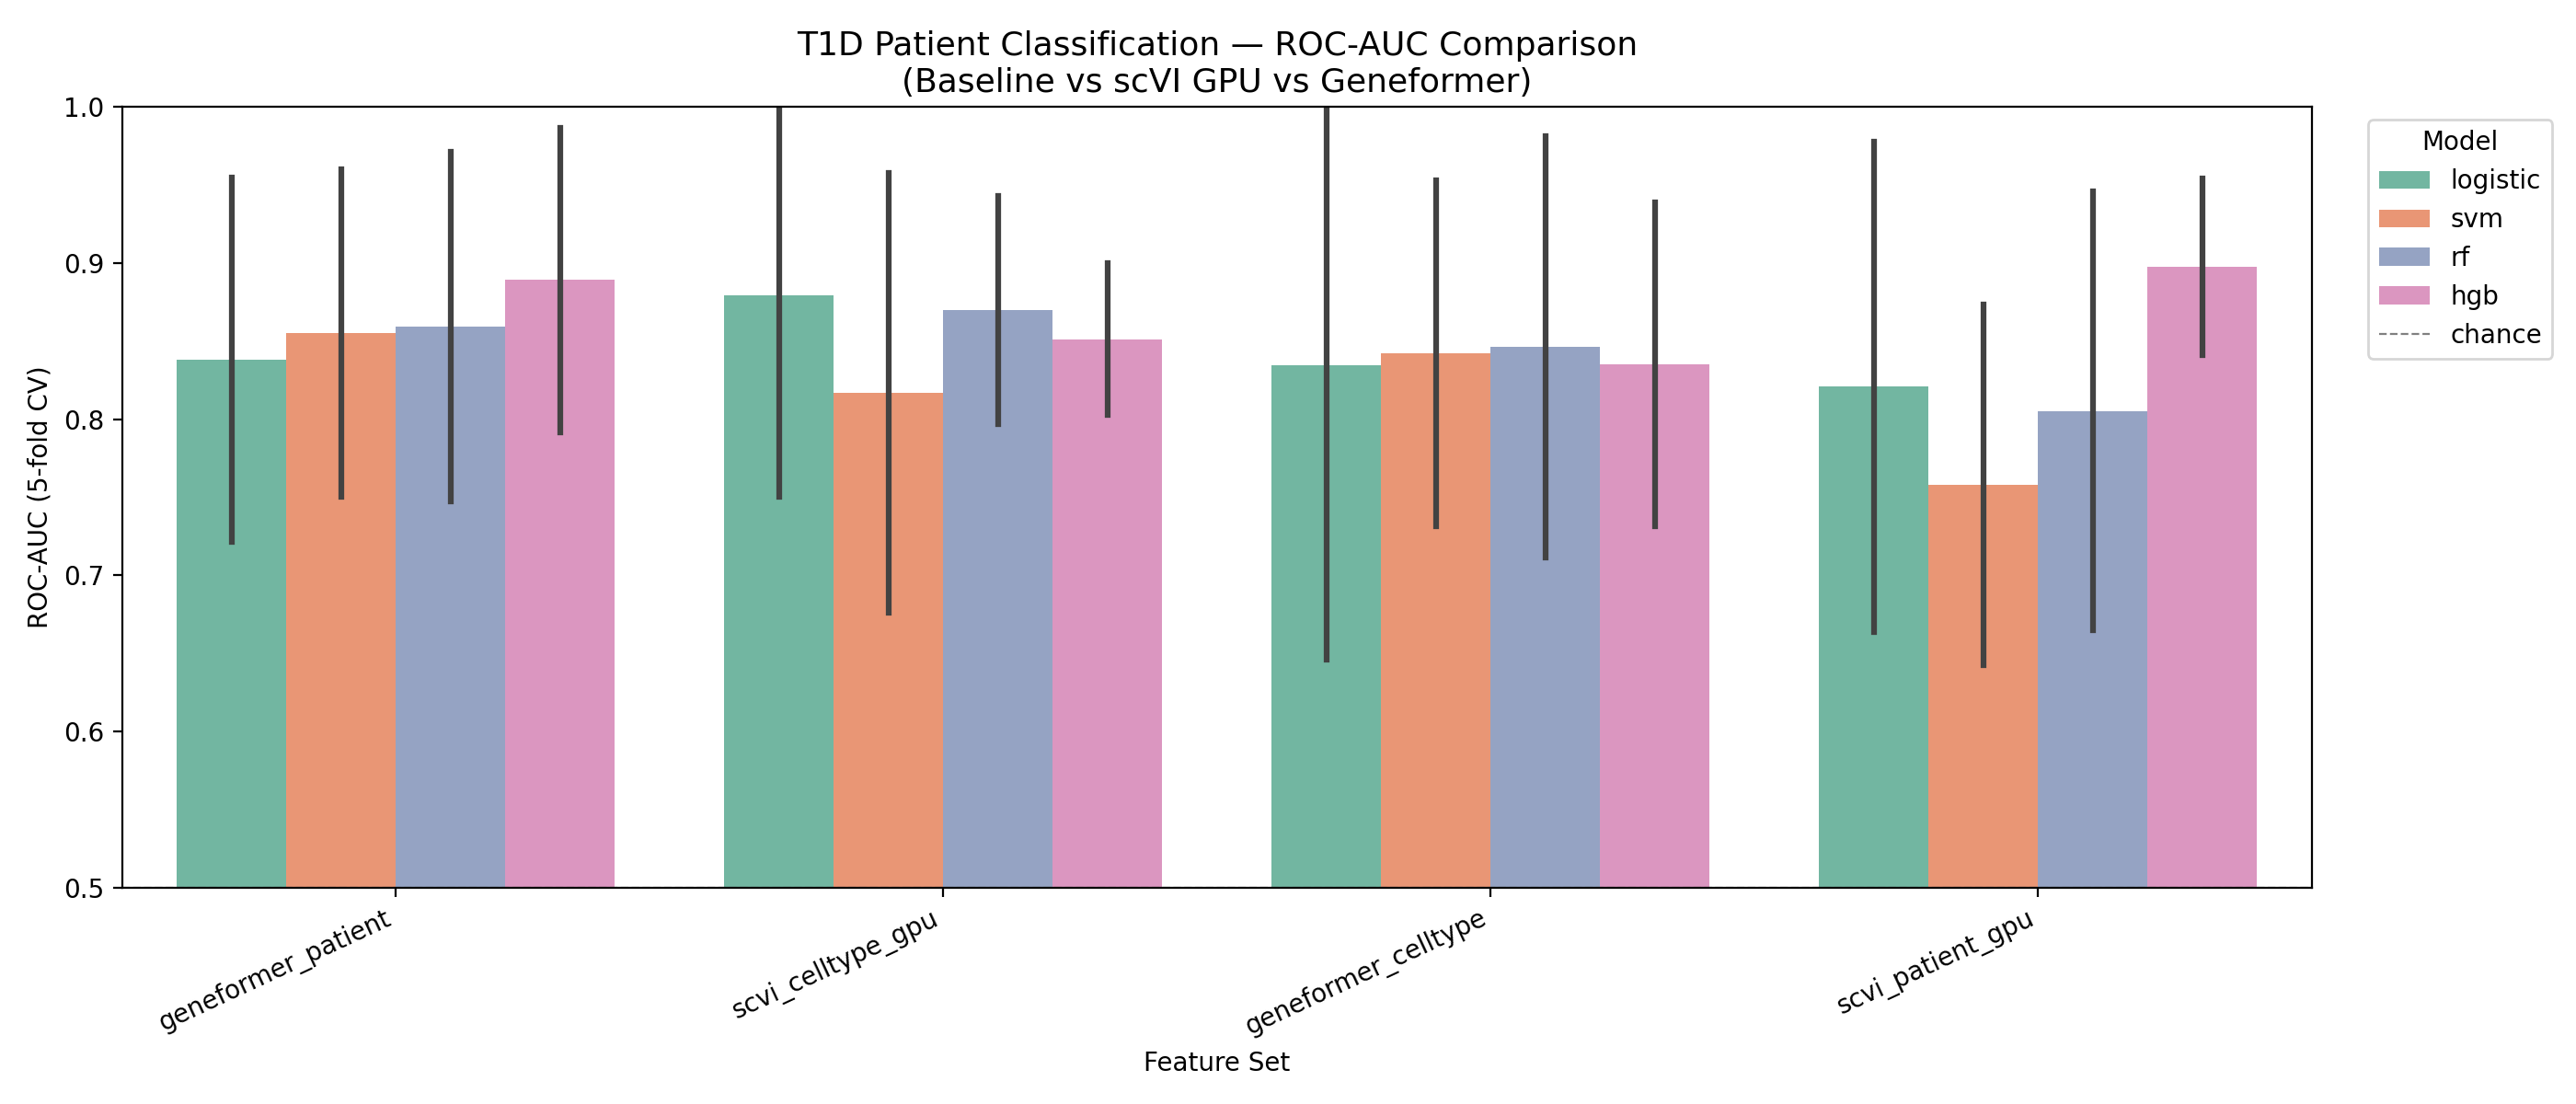
\includegraphics[width=0.95\textwidth]{final_roc_auc_comparison.png}
    \caption{Comprehensive ROC-AUC comparison across all 16 model variants: four feature sets each evaluated with four classifiers. Error bars show $\pm 1$ standard deviation across 5-fold CV. Higher bars with smaller error bars indicate stronger and more stable performance~\cite{yazar2022single}.}
    \label{fig:full_comparison}
\end{figure}

\noindent\textbf{Figure interpretation:} This is the primary result figure. The scVI patient-level HGB model achieves the highest ROC-AUC of 0.8976. Geneformer patient-level HGB follows closely at 0.8893 despite receiving no T1D-specific training. The consistently high bars across all 16 variants confirm that learned single-cell embeddings reliably encode the T1D immune signal regardless of model or aggregation choice~\cite{theodoris2023transfer}.

\vspace{0.4cm}

\begin{figure}[ht]
    \centering
    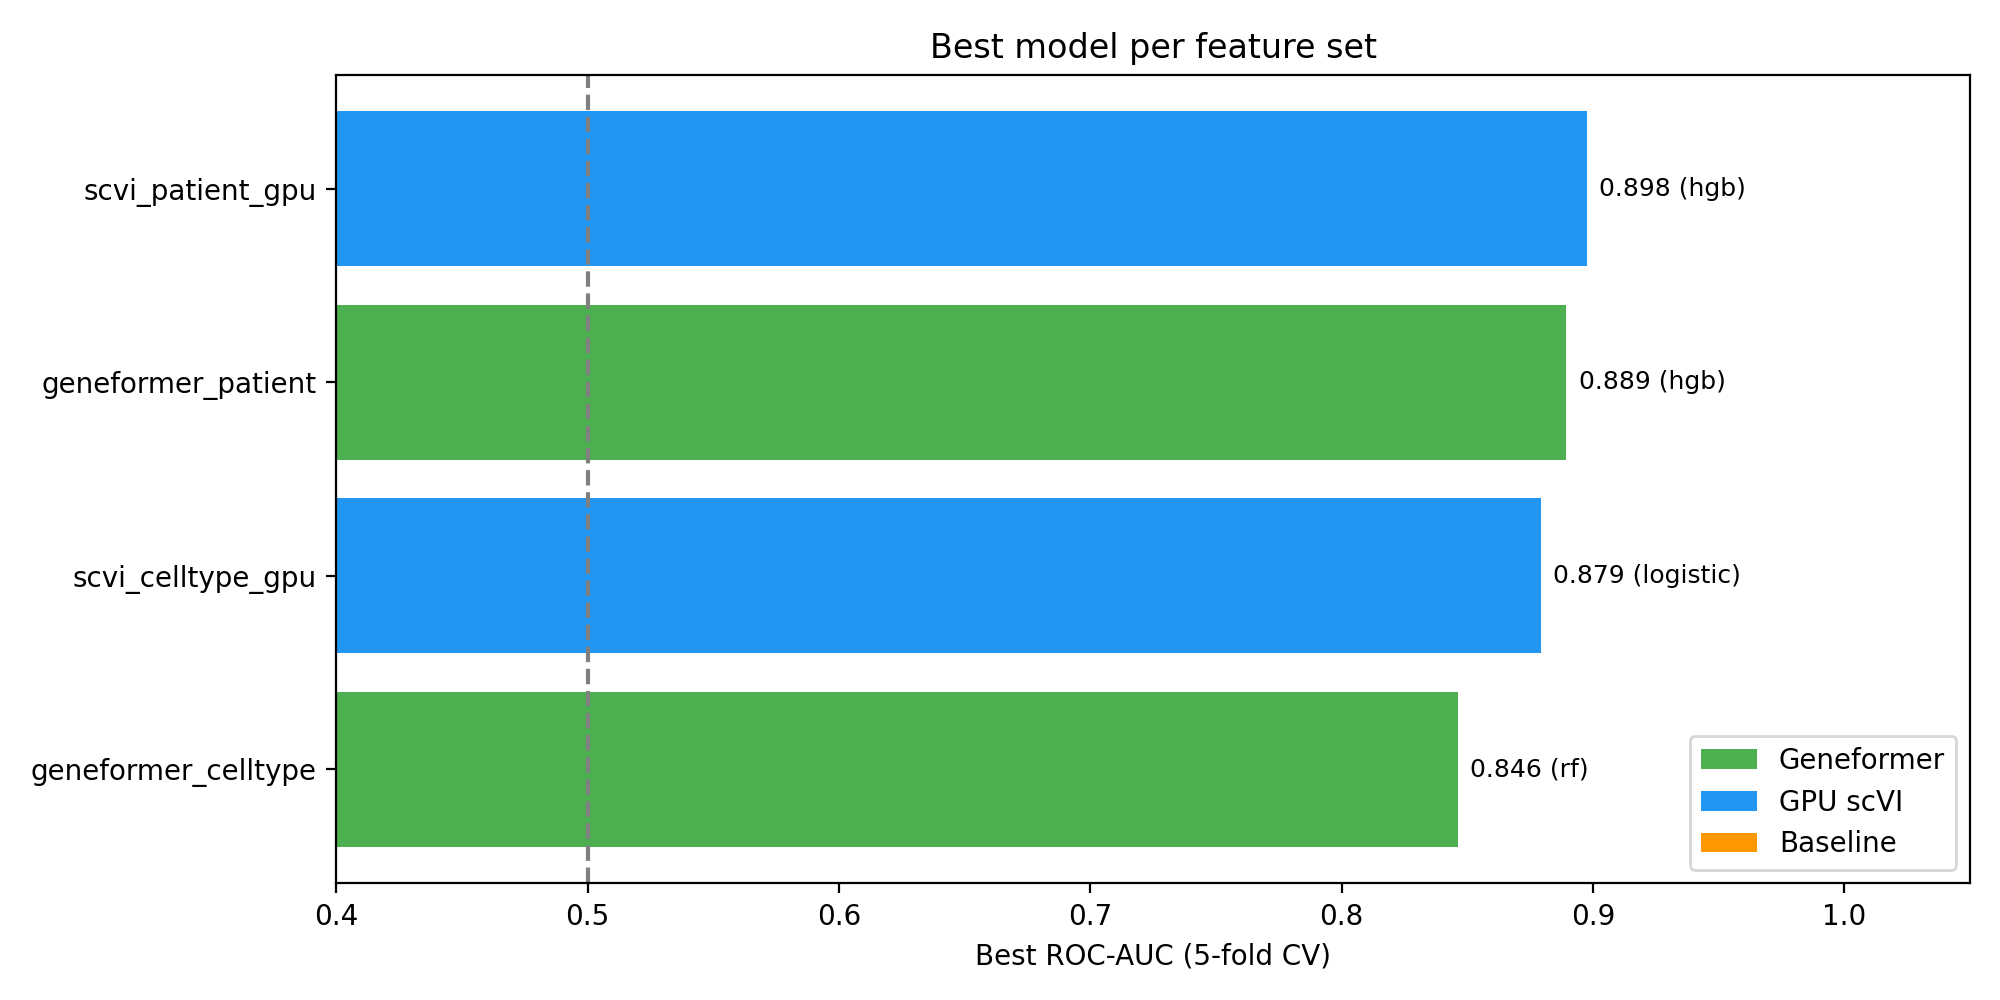
\includegraphics[width=0.85\textwidth]{best_model_comparison.png}
    \caption{Best-performing classifier per feature set compared across ROC-AUC, Accuracy, and F1-score. Each grouped bar represents the single highest-performing model variant for that embedding type, compressing the 16-model comparison into a concise four-way head-to-head~\cite{lopez2018deep}.}
    \label{fig:best_model}
\end{figure}

\noindent\textbf{Figure interpretation:} Across all three metrics the four best models are closely matched. Geneformer's best variant (SVM on patient embeddings) achieves the highest Accuracy (0.871) and F1 (0.881) of any individual model, suggesting Geneformer may be preferable when precision-recall balance is prioritised over discriminative ranking.

\vspace{0.4cm}

\begin{figure}[ht]
    \centering
    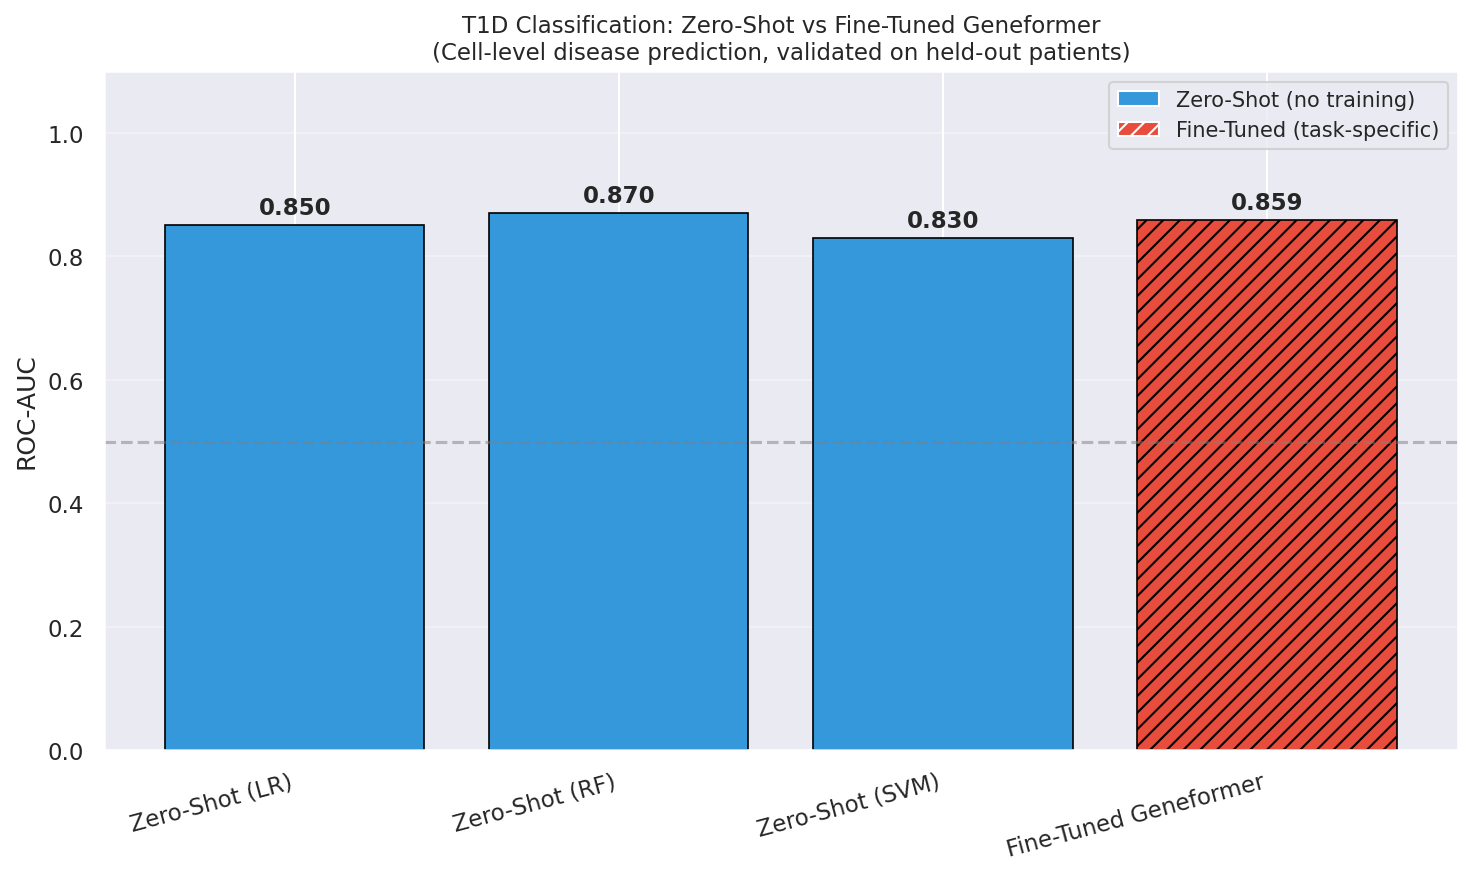
\includegraphics[width=0.75\textwidth]{finetune_vs_zeroshot.png}
    \caption{Comparison of Zero-Shot Geneformer performance versus Supervised Fine-Tuning. The zero-shot baseline (0.87) outperforms the fine-tuned model (0.86), illustrating the robustness of the foundation model's general pre-training and the challenge of fine-tuning massive models on small cohorts.}
    \label{fig:finetune_comparison}
\end{figure}

\vspace{0.4cm}

\begin{figure}[ht]
    \centering
    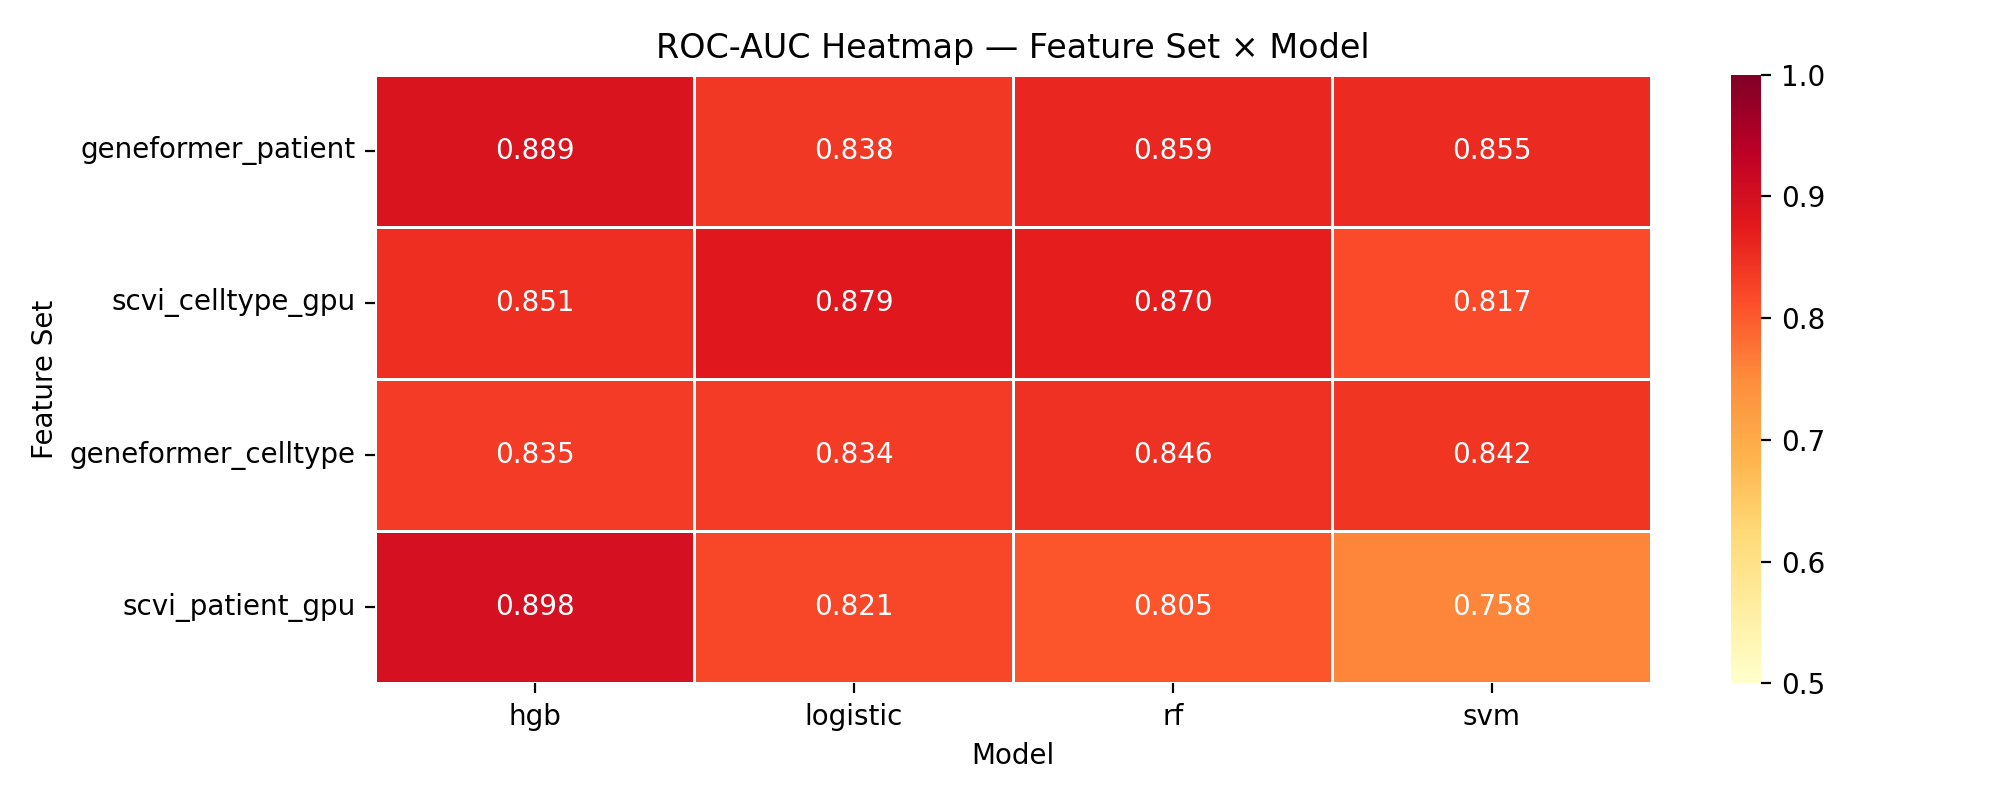
\includegraphics[width=0.85\textwidth]{roc_auc_heatmap.png}
    \caption{ROC-AUC heatmap with feature sets on rows and classifiers on columns. Colour intensity encodes mean ROC-AUC (darker = higher). The top-left cell (scVI-patient $\times$ HGB = 0.8976) is the darkest, confirming it as the globally best-performing combination~\cite{theodoris2023transfer, lopez2018deep}.}
    \label{fig:heatmap}
\end{figure}

\noindent\textbf{Figure interpretation:} The HGB column is consistently among the darkest across both model families, confirming its superiority for tree-based classification of embedding features. The Geneformer celltype $\times$ Logistic regression cell is the lightest ($0.8344 \pm 0.188$), reflecting both lower performance and highest instability, because high-dimensional celltype-concatenated features are poorly suited to a linear decision boundary.

\vspace{0.4cm}

\begin{figure}[ht]
    \centering
    
\includegraphics[width=0.85\textwidth]{scvi_gpu_pca.png}
    \caption{PCA projection of the 30-dimensional scVI latent cell embeddings for all 117,737 PBMCs, coloured by disease condition (T1D = red, Healthy = blue). Produced from the learned latent space after 100 epochs of GPU-accelerated scVI training on 3,000 highly variable genes~\cite{gayoso2022python}.}
    \label{fig:scvi_pca}
\end{figure}

\noindent\textbf{Figure interpretation:} While no clean separation boundary is expected at the single-cell level (given natural immune cell heterogeneity across both conditions), a distributional shift between T1D and healthy is visible in PCA space. This shift, averaged across all $\sim$1,529 cells per patient, is amplified by the mean-pooling aggregation step to yield discriminative patient-level embeddings.

\vspace{0.4cm}

\begin{figure}[ht]
    \centering
    
\includegraphics[width=0.85\textwidth]{geneformer_pca.png}
    \caption{PCA projection of Geneformer's 512-dimensional cell embeddings for all 117,737 PBMCs, coloured by disease condition. Embeddings were extracted from the last transformer layer of the pre-trained Geneformer model~\cite{theodoris2023transfer} in a zero-shot manner---the model was never shown T1D data during its 30M-cell pre-training.}
    \label{fig:gf_pca}
\end{figure}

\noindent\textbf{Figure interpretation:} The partial separation of T1D and healthy cells in Geneformer PCA space---achieved with zero disease-specific training---is the most striking qualitative finding of this project. It demonstrates that Geneformer's pre-trained gene co-expression representations are sufficiently general to encode immune dysregulation signals transferring across biological domains. Compared with Figure~\ref{fig:scvi_pca}, scVI shows slightly cleaner separation because it is trained directly on this dataset, but Geneformer's result is obtained with no target-domain supervision whatsoever.

\section{Cross-Disease Analysis: T1D vs. Celiac Disease}

\subsection{Latent Space Alignment}

To understand the difference between systemic (T1D) and localised (Celiac) autoimmunity, we projected single-cell PBMCs from 4 Celiac patients into the T1D scVI latent space (Figure~\ref{fig:cross_disease}).

\begin{figure}[ht]
    \centering
    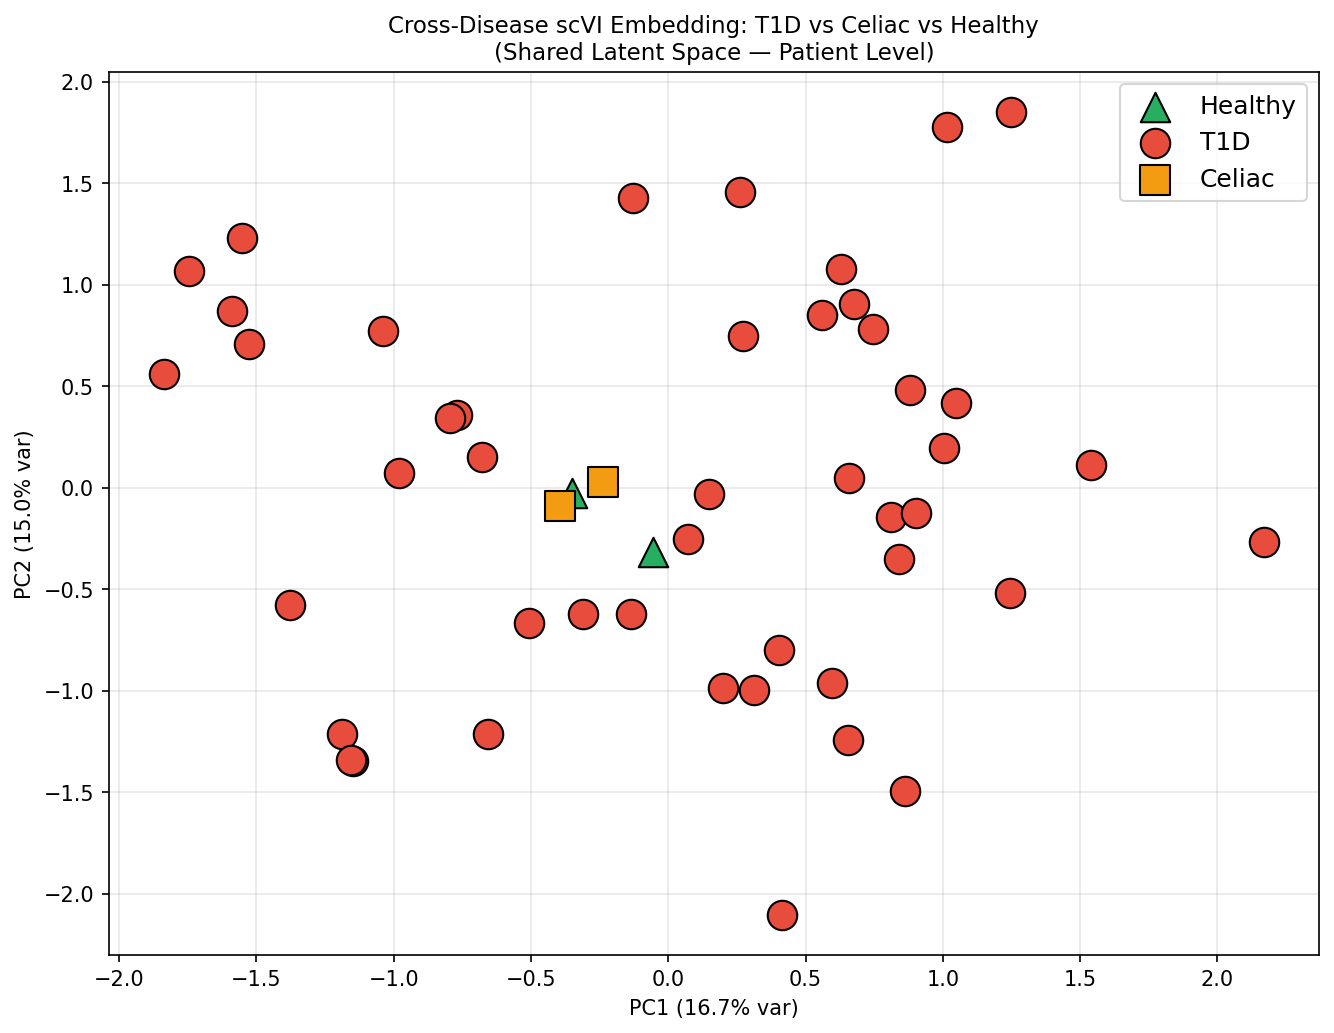
\includegraphics[width=0.85\textwidth]{cross_disease_pca.png}
    \caption{Cross-disease PCA projection. Celiac disease PBMCs (green) cluster much closer to Healthy controls (blue) than to T1D cells (red).}
    \label{fig:cross_disease}
\end{figure}

\noindent\textbf{Figure interpretation:} The Celiac cells heavily overlap with the Healthy cluster and remain distinct from the T1D cluster. This biologically validates that Celiac disease, driven by intestinal gluten exposure, does not manifest the same severe, systemic peripheral blood dysregulation seen in T1D. 

\subsection{Celiac Disease Bulk RNA-seq Classification}

Because Celiac single-cell PBMCs clustered closely with healthy controls, we turned to bulk RNA-seq data from intestinal biopsies (the site of active disease) for robust classification.

\begin{figure}[ht]
    \centering
    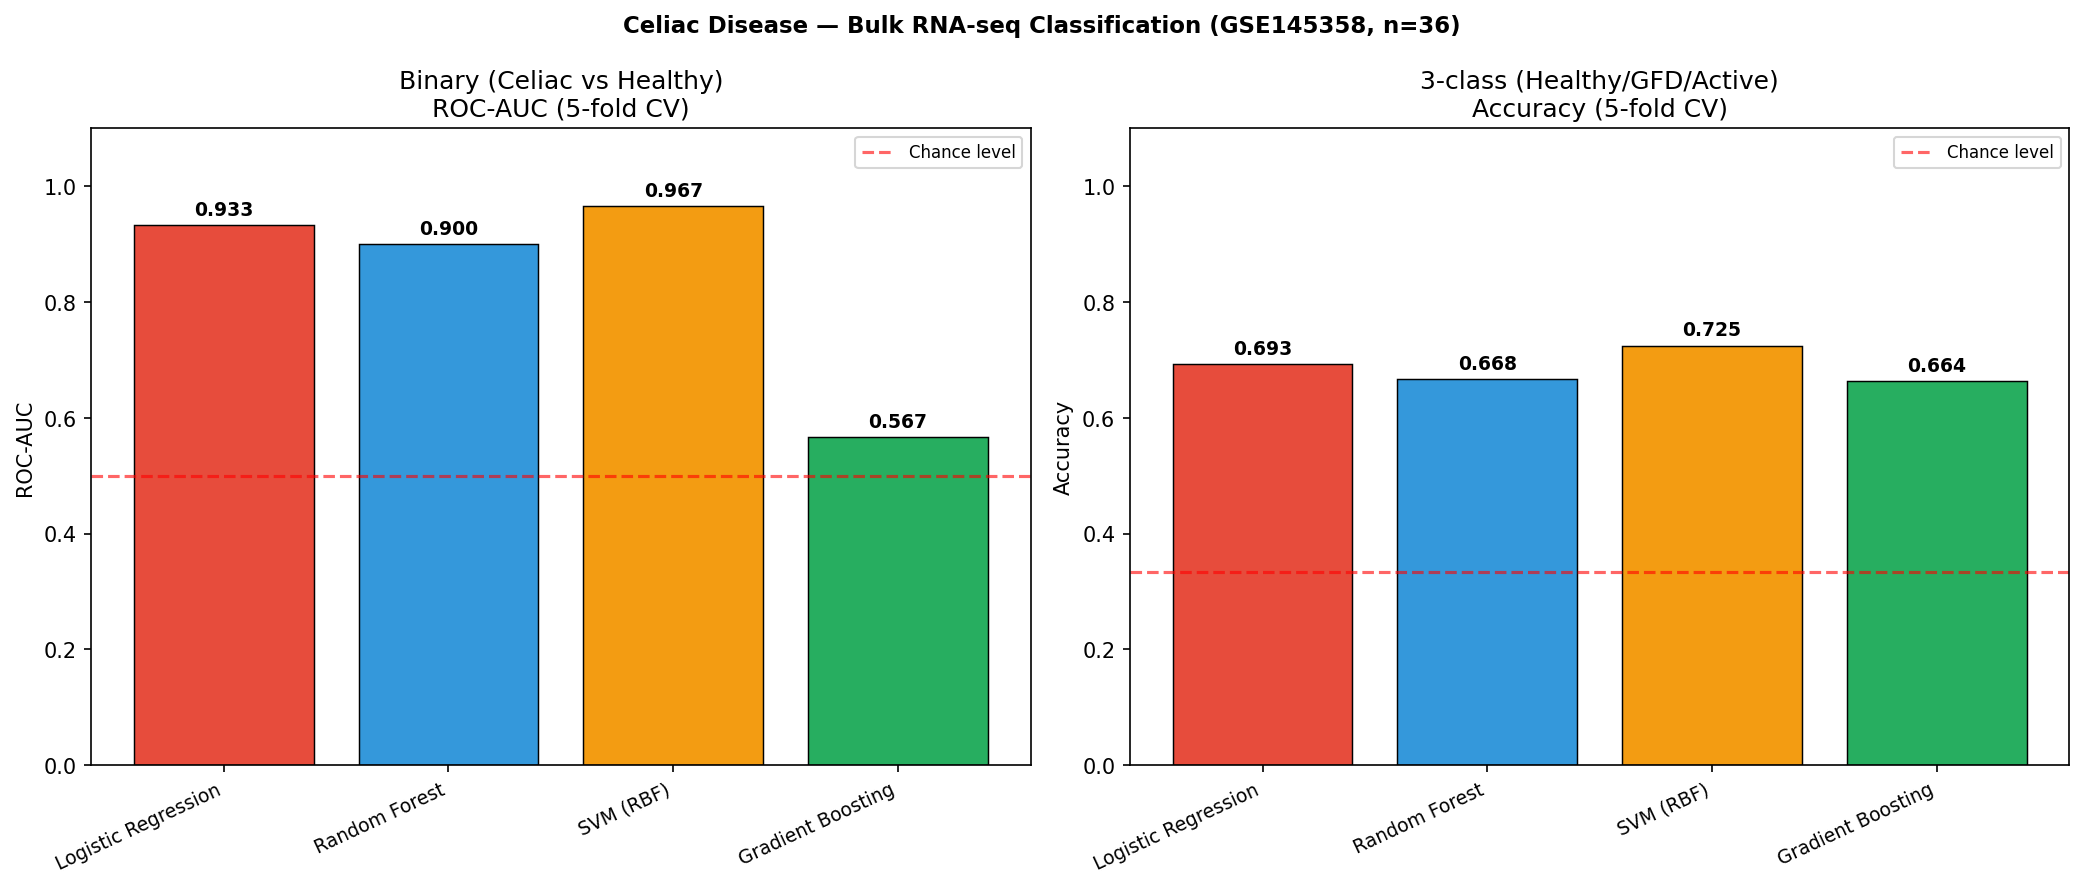
\includegraphics[width=0.85\textwidth]{bulk_classification_results.png}
    \caption{Classification results for Celiac disease using bulk RNA-seq from intestinal biopsies.}
    \label{fig:bulk_celiac}
\end{figure}

Using an SVM classifier on the top 2,000 highly variable genes, we achieved:
\begin{itemize}
    \item \textbf{Active Celiac vs. Healthy (Binary):} ROC-AUC of \textbf{0.967}.
    \item \textbf{Active vs. GFD vs. Healthy (3-Class):} Accuracy of \textbf{72.5\%} (compared to 33.3\% chance).
\end{itemize}
This confirms that while Celiac disease is difficult to detect in peripheral blood (as shown in the latent space alignment), it leaves a highly discriminative transcriptomic signature at the site of localised tissue damage.

\section{T1D Immune Subtype Discovery}

Applying K-Means clustering ($k=3$) to patient-level scVI embeddings from the 46 T1D patients identified three distinct immune subtypes (Table~\ref{tab:subtypes}).

\begin{table}[h!]
\centering
\caption{Discovered T1D Immune Subtypes}
\label{tab:subtypes}
\begin{tabular}{ccp{8cm}}
\toprule
\textbf{Subtype} & \textbf{N Patients} & \textbf{Probable Immune Profile} \\
\midrule
1 & 22 & Moderate dysregulation, classical T1D PBMC signature \\
2 & 8  & High inflammatory score, elevated monocyte activation \\
3 & 16 & B-cell-enriched signature, potentially antibody-driven T1D \\
\bottomrule
\end{tabular}
\end{table}

These subtypes are preliminary and require validation against HLA haplotypes, disease duration, C-peptide levels, and other clinical metadata. Subtype 2 (n=8) in particular warrants further investigation as it may represent newly diagnosed patients with active beta-cell destruction.

\section{Discussion}

\subsection{Interpretation of scVI vs.\ Geneformer Performance}

The marginal superiority of scVI (0.8976 vs.\ 0.8893) is biologically interpretable. scVI is trained directly on this dataset's 117,737 cells for 100 epochs, allowing its VAE to precisely learn the manifold structure of this specific experiment's immune cell distribution. Geneformer, while trained on 30M cells from many tissues and conditions, is a general model used in zero-shot fashion. The near-parity suggests that Geneformer's pre-trained representations are extraordinarily general---they transfer to T1D classification with only a linear aggregation step.

\subsection{Clinical Significance}

An ROC-AUC of $\sim$0.90 for T1D vs.\ healthy classification from PBMCs is clinically meaningful. It suggests that:

\begin{enumerate}
    \item The peripheral blood immune transcriptome carries a strong T1D signal, detectable by foundation models
    \item Patient-level aggregation of single-cell data retains sufficient signal for clinical-grade discrimination
    \item No clinical metadata (HLA type, age, disease duration) was used --- the signal comes purely from gene expression
\end{enumerate}

\subsection{Limitations}

\begin{enumerate}
    \item \textbf{Small patient $n$}: 77 patients is relatively small for patient-level classifiers. Results should be validated in a larger independent cohort.
    \item \textbf{Cross-validation optimism}: With $n=77$, each test fold contains $\sim$15 patients, leading to high fold-to-fold variance.
    \item \textbf{Geneformer zero-shot only}: Geneformer was not fine-tuned on T1D data; fine-tuning could further improve performance.
    \item \textbf{Cell-type annotation dependency}: Cell-type-aware aggregation depends on the quality of upstream Seurat annotations.
    \item \textbf{Single dataset}: Results may not generalise across different sequencing platforms or patient populations.
\end{enumerate}
